\documentclass{article}
\usepackage[english]{babel}
\usepackage[a4paper,top=2.54cm,bottom=2.54cm,left=2.54cm,right=2.54cm]{geometry}
\usepackage{amsmath}
\usepackage{graphicx}
\usepackage[colorlinks=true, allcolors=blue, citecolor=black]{hyperref}
\usepackage{apacite}
\usepackage[utf8]{inputenc}
\usepackage{setspace} 
\doublespacing{}
\usepackage[singlelinecheck=false,justification=justified]{caption}
\usepackage{listings}
\usepackage{xcolor}
\usepackage{floatrow}
\floatsetup[figure]{capposition=top}
\definecolor{codegreen}{rgb}{0,0.6,0}
\definecolor{codegray}{rgb}{0.5,0.5,0.5}
\definecolor{codepurple}{rgb}{0.58,0,0.82}
\definecolor{backcolour}{rgb}{0.95,0.95,0.92}
\lstdefinestyle{mystyle}{
  frame=shadowbox,
  backgroundcolor=\color{backcolour},   commentstyle=\color{codegreen},
  keywordstyle=\color{magenta},
  numberstyle=\tiny\color{codegray},
  stringstyle=\color{codepurple},
  basicstyle=\ttfamily\footnotesize,
  breakatwhitespace=false,         
  breaklines=true,                 
  captionpos=b,                    
  keepspaces=true,                 
  numbers=left,                    
  numbersep=5pt,                  
  showspaces=false,                
  showstringspaces=false,
  showtabs=false,                  
  tabsize=2
}
\lstset{style=mystyle}

\newcommand\blfootnote[1]{
\begingroup
\renewcommand\thefootnote{}\footnote{#1}
\addtocounter{footnote}{-1}
\endgroup
}
\date{\parbox{\linewidth}{\centering%
  \today\endgraf\bigskip
  Advanced Databases – TU60 2021/2022 - Brendan Tierney}}
\title  {Assignment A: Amazon Aurora DB}
\author{Rodrigo Antonio Costa Tavares - D20125370}
\begin{document}
\maketitle
\thispagestyle{empty}
\begin{abstract}

\noindent Cloud Computing has been becoming the default go-to model for IT as companies are prioritizing on demand service providers over traditional vendors to accelerate digital transformation projects, when it comes to relational databases in public clouds, Amazon Aurora DB is the most used Cloud database engine compatible with MySQL and PostgreSQL. Aurora is provided by AWS (Amazon Web Services) through the Amazon Relational Database Service (RDS) which is a managed service that offers databases in the cloud. This study has demonstrated some of the RDS Aurora capabilities as creating a MySQL RDS in the cloud, Working with Read Replica capabilities, Common DBA tasks for MySQL DB instances, terminating  the environment in the cloud, the importance of Aurora and managed services as RDS for the enterprise, technical considerations around Aurora MySQL and Aurora PostgreSQL, the historical evolution of Aurora DB, alternatives and comparisons with Google Cloud SQL and Azure SQL Database. 
This study has demonstrated successfully how AWS RDS Aurora DB is suitable and ready for the enterprise, and has identified the AWS service as one of the best options available in the market, apart from some specific workloads that are better handled by other providers, and some drawbacks identified, AWS RDS Aurora is still the most mature option among those evaluated to run MySQL and PostgreSQL in the Cloud. 

\noindent \textbf{Key words:} Databases, Cloud, Replication, Cluster, Instance, MySQL, PostgerSQL, Security, DBA, Comparison, Demonstration

\end{abstract}

\clearpage
\tableofcontents
\clearpage
\listoffigures
\clearpage

\section{Introduction}

Amazon Aurora DB is an enterprise relational database engine compatible with MySQL and PostgreSQL. Aurora is provided by AWS (Amazon Web Services) through the Amazon Relational Database Service (RDS) which is a managed service that serves databases in the cloud, with RDS customers shares the responsibility of maintaining the database underline infrastructure with Amazon\cite{todorov2013aws}.

In the following pages, we will demonstrate the Amazon Aurora capabilities, the importance of Aurora and managed services as RDS for the enterprise, technical considerations around Aurora MySQL and Aurora PostgreSQL.  We will also see alternatives and comparisons that will allow us to understand the difference between Amazon RDS and Amazon Aurora. Finally, I will demonstrate how to deploy a sample database and how to create a DB Cluster using AWS RDS Aurora with MySQL and Terraform, at the end of this demonstration we will be able to see the main functionalities and how it compares with traditional databases.

\section {Aurora DB Background, Importance and Technical Details}

Aurora is ultimately a new version of AWS RDS. The engineering behind Aurora is a unique approach that was recognized and awarded in 2019 the SIGMOD Systems Award where the developers of Aurora won the award for fundamentally redesigning relational database storage for cloud environments \cite{sigmod2021}. 

AWS in their public documentation defines Amazon RDS as a Relational Database Service (Amazon RDS) that makes it easier to set up, operate, and scale a relational database in the AWS Cloud. In this session we will have a look in the importance and technical details about Aurora, it's main capabilities of AWS Aurora as Auto-scaling, Backup/restore, High Availability and Replication, Monitoring and Security and at the end there will be a tutorial for those who want to follow along the demonstration we will be doing. 

\subsection{What won't be covered in this study, Research limitations}

The focus of this demonstration is to illustrate the Amazon Aurora capabilities, so we won’t be investing time in configuration, installation, and tooling, it’s expected that the reader is already familiarized with the basic tools that allow the interaction with the cloud, however, the links and references for each pre-requirement tasks will be provided so anyone with internet access and an AWS account can replicate the same steps.

It's important to highlight that even though MariaDB is a fork of the MySQL open source project, the AWS RDS serive object of this study is based only on MySQL, AWS has a different offer called Amazon RDS for MariaDB that won't take part in this research. 

Cloud computing in 2021 has become the go-to model for IT as companies prioritize on demand service providers over traditional vendors in order to be able to accelerate digital transformation projects, and enable the new normal of work following the COVID-19 pandemic \cite{dignan2021}. There is a massive run leaded by the main cloud providers and their products are constantly changing, while this study was been written, new features and capabilities have been added to the managed, on top of it the service itself is massive, a number of different features and capabilities are not part of the scope of this study:  

\begin{itemize}
    \item An active AWS account is required in order to deploy the lab environment used in the Demonstration and it can take time to activate a new account. \cite{createaccount}. 
    \item MariaDB will not be covered. 
    \item The comparison with Alternative Solutions and Traditional Technologies might not be precise due to new features constantly being added to the products.\cite{rdsvsazure2019} 
    \item Amazon Aurora Serverless is nor part of the scope of this study. 
    \item For the propose of this study only DB Instance will be used, Aurora DB clusters won't be covered in our demonstration, DB instance will be used instead.
    \item MySQL Database Service in Oracle Cloud
\end{itemize}
 
\subsection{Amazon Aurora DB clusters vs DB Instances}    

Most of the AWS services will be offered in form of single instances of the service when the service is deployed in only one Availability Zone with no replicas spread across other zones or regions and also in cluster mode where multiple instances of the service will be provided across multiple availability zones to provide high availability,  when it comes to enterprise solutions the Aurora DB cluster where multiple instances and a cluster volume that manages the data for those DB instances are provided to serve the database endpoint, the cluster volume is a virtual storage volume used by the database that spans multiple Availability Zones, with each Availability Zone having a copy of the cluster data. Any Aurora DB Cluster have at least two types of DB instances \cite{amazon2006amazon}:

\begin{itemize}
    \item Primary DB instance – Supports read and write operations, and performs all of the data modifications to the cluster volume. Each Aurora DB cluster has one primary DB instance.
    \item Aurora Replica – Connects to the same storage volume as the primary DB instance and supports only read operations. Each Aurora DB cluster can have up to 15 Aurora Replicas in addition to the primary DB instance. Maintain high availability by locating Aurora Replicas in separate Availability Zones. Aurora automatically fails over to an Aurora Replica in case the primary DB instance becomes unavailable. You can specify the failover priority for Aurora Replicas. Aurora Replicas can also offload read workloads from the primary DB instance \cite{dbcluster2021}.
\end{itemize}

The following diagram illustrates the relationship between the cluster volume, the primary DB instance, and Aurora Replicas in an Aurora DB cluster. As illustrated in the previous session, for the propose of the demonstration we will be executing in the following sessions, only the DB instance will be used. 

\begin{figure}[hbt!]
\centering
\caption{\label{fig:dbcluster} Amazon Aurora DB Cluster}
\fbox{\includegraphics[width=0.9\textwidth]{AuroraArch001.png}}
\floatfoot{\cite{dbcluster2021}}
\end{figure}

For the propose of the demonstration 
\subsection{AWS Database Architecture in Aurora}

AWS resources are hosted in multiple locations world-wide, these locations are composed of AWS Regions, Availability Zones, and Local Zones \ref{fig:awszones}. Each AWS Region is a separate geographic area and each AWS Region has multiple, isolated locations known as Availability Zones, in our demonstration we will be using two different local zones so if single location is affected by any failure, none of our DB instances will be affected \cite{awszones}. 

\begin{figure}[hbt!]
\centering
\caption{\label{fig:awszones} RDS Regions, Availability Zones, and Local Zones.}
\fbox{\includegraphics[width=0.9\textwidth]{zones.png}}
\floatfoot{Note. Each AWS Region is designed to be isolated from the other AWS Regions. This design achieves the greatest possible fault tolerance and stability \cite{awszones}}
\end{figure}

This design allows Amazon to provide high availability and failover support for DB instances using Multi-AZ deployments. Differently from the native MySQL and PostgreSQL High availability tools, Multi-AZ deployments in Aurora use Amazon's failover technology \cite{awsha}.

\subsection{Aurora DB MySQL}
The first MySQL version appeared in 1995 released by Michael Widenius and Swedes David Axmark, MySQL is a open-source database under the terms of the GNU General Public License, the database was developed for many years by the company	MySQL Ab, which was acquired in 2008 by Sun	Microsystems, that in turn,	acquired by	Oracle	Corporation one year later,	in	2009. The day Oracle announced the purchase of Sun, Michael Widenius forked MySQL, launching MariaDB, and took a part of MySQL developers with him \cite{bartholomew2012mariadb}.

It's important to highlight that even though MariaDB is a fork of the MySQL open source project, the AWS RDS offer object of this study is based only on MySQL, AWS has a different offer called Amazon RDS for MariaDB that won't take part in this research. 

\subsection{Aurora DB PostgreSQL}

According to \cite{perkins2018seven} PostgreSQL is the finest open source example of the relational database management system (RDBMS) tradition, re-branded in 1996, it's roots are considerably older as the original project was written at Berkeley in the early 1970s with the name of "Ingres". it supports transactions with Atomicity, Consistency, Isolation, Durability (ACID) properties. In November 2016, Amazon Web Services announced the addition of PostgreSQL compatibility to their cloud-native Amazon Aurora managed database offering. 

Among the mai capabilities offered to RDS PostgreSQL, we can highlight the AWS Database Migration Service (DMS), which integrates RDS to migrate Databases. DMS reads an existing database setup, translates it to PostgreSQL, and imports it into an RDS instance, below we can see a list of other capabilities of RDS PostgreSQL: 

\begin{itemize}
    \item Scale PostgreSQL up and down with AWS native capabilities. 
    \item Automatic replication for high available and redundancy. 
    \item Switching to RDS + PostgreSQL with AWS DMS;. 
    \item Easy to setup and restore databases backups using snapshots. 
\end{itemize}


\subsection{Why Amazon Aurora is important for enterprises?}
According to \cite{dbengineers2021}, MySQL and PostgreSQL are among the 4 most popular DMS (Database Management Systems) in the world with MySQL in 2nd and PostgreSQL in 4th as shown in Figure \ref{fig:DBRanking}. These two DMS together are widely adopted in enterprise organizations as the biggest representatives of the open-source databases engines, and they have been around even before the advent of cloud computing. 

\begin{figure}[hbt!]
\centering
\caption{\label{fig:DBRanking}DB-Engines Ranking, October 2021.}
\fbox{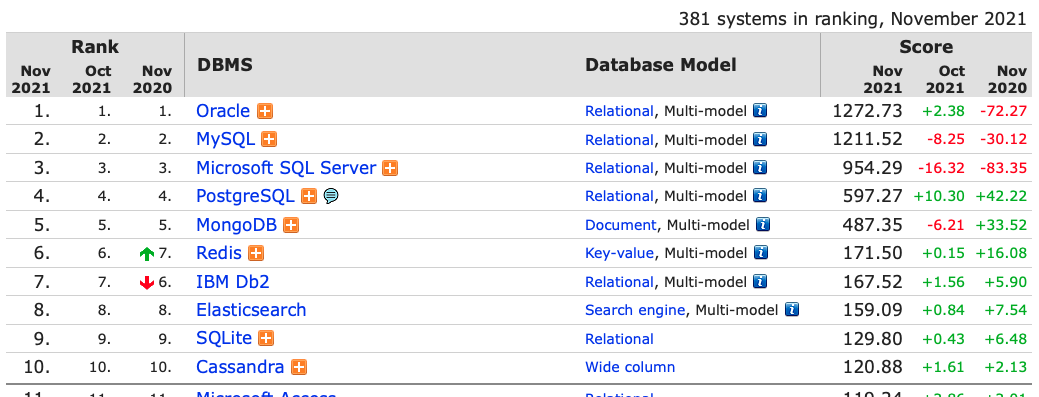
\includegraphics[width=0.9\textwidth]{dbrank.png}}
\floatfoot{Note. MySQL and PostgreSQL are the only databases to presented an expressive growth in Sep 2021.}
\end{figure}

Amazon Aurora was released in October 2014 supporting only MySQL, since then the managed service has been updated following the MySQL and MariaDB community, this proximity with the opensource is important for enterprises since their workload for databases is still being held in on-premises data centers, Aurora DB is important not only for those who want to migrate their databases to the cloud but even more important for new companies, startups with MySQL and PostgreSQL that don’t want to expend time and money in building data centers to host their solutions. Cloud is flexible and scalable it helps with business continuity and disaster recovery, and drives collaboration and efficiency in a way that new companies cannot afford, building infrastructure spread around the world with smart services is not an easy task \cite{mihalec2021}

\subsection{The evolution of Aurora DB over the past 7 years }

On 12th November 2014, AWS announced Amazon Aurora as the MySQL compatible Amazon Relational Database Service (RDS) that was launched in 2009, at the time the service was designed for 99.99\% availability and mechanisms that allowed automatically recovery from instance and storage failures according to \cite{jeffbarr2014}, over the time new features and capabilities were added. Let’s see now Aurora DB has evolved in this past almost 8 years. 

Thankfully AWS keeps a documented history for their services from where we can follow important changes to the products, for the proposal of this academic work I have created the Figure \ref{fig:AmazonAuroraOverTheYears} based on the Aurora DB Document History \cite{awsdocumentedhistory} that allows us to see the evolution of Aurora DB over the past 7 years:

\begin{figure}[hbt!]
\centering
\caption{\label{fig:AmazonAuroraOverTheYears}The evolution of Aurora DB over the past 7 years }
\fbox{\includegraphics[width=0.9\textwidth]{AmazonAuroraOverTheYears.png}}
\floatfoot{Note. Before August 31, 2018, Amazon Aurora was documented in the Amazon Relational Database Service User Guide. For earlier Aurora document history, see Document history in the Amazon Relational Database Service User Guide.}
\end{figure}
\clearpage

\section{Aurora DB Tutorial Demonstration with MySQL}

The focus of this demonstration is to illustrate the Amazon Aurora capabilities, so we won’t be investing time in configuration, installation, and tooling, it’s expected that the reader is already familiarized with the basic tools that allow the interaction with the cloud, however, the links and references for each pre-requirement tasks will be provided so anyone with internet access and an AWS account can replicate the same steps.

Before you proceed, please have in mind that we will be using the AWS free tier for Amazon RDS which provides 750 hours of RDS single-AZ db.t2.micro instance using MySQL or MariaDB with 20GB for storage and 20GB for storage backups (Amazon, 2021), if you follow strictly the instructions in this session, you should not be charged for the deployed resources if they are the only one resources you have in your account at the moment you terminate the lab, if you destroy the resources right after completing the laboratory, no charges should be implied, however, stick to the idea that moving on with this laboratory is your entire responsibility :
In order to be able to create an Amazon Aurora Database in AWS, you will need to first:

\begin{enumerate}
\item Create and activate an AWS account if you don’t have one, please refer to the article "How do I create and activate a new AWS account?" \cite{createaccount}
\item Install Tettaform \cite{installterraform}. 
\item Install AWS CLI  \cite{installawscli}
\item Configure AWS Credentials \cite{configurecredentials}
\end{enumerate}

\subsection{Architecture}
When it comes to the difference architectures being implemented in on-premises environments and public clouds, it's not surprising how similar they can be with each other. Lets imagine we are building a computing environment to host databases, the tables will not magically appear in a console with an endpoint to where you can send SQL queries, we will need hardware, computing resources, networking, etc. In the cloud is not that different, but there you won't need to buy directly this resources, install and configure them, the cloud provider have done that for you, and they will charge you based on the amount of resources you consume according to the agreement you have made. 

Let's try to approach each of the components of this architecture starting by the networking, every AWS account has a Default VPC (Virtual Private Cloud) which is responsible for managing all the aspects of your the network, you can imagine a VPC as the service that will limit the scope of your private network, and consequently your applications, databases and services, we will be using the Defaut VPC to host the Web application, for the propose of this demonstration. As we can see in the image below the VPC is what separates our private network from the internet. 

\begin{figure}[hbt!]
\centering
\caption{\label{fig:Arqchitecture} Demonstration Architecture with Bastion host.}
\fbox{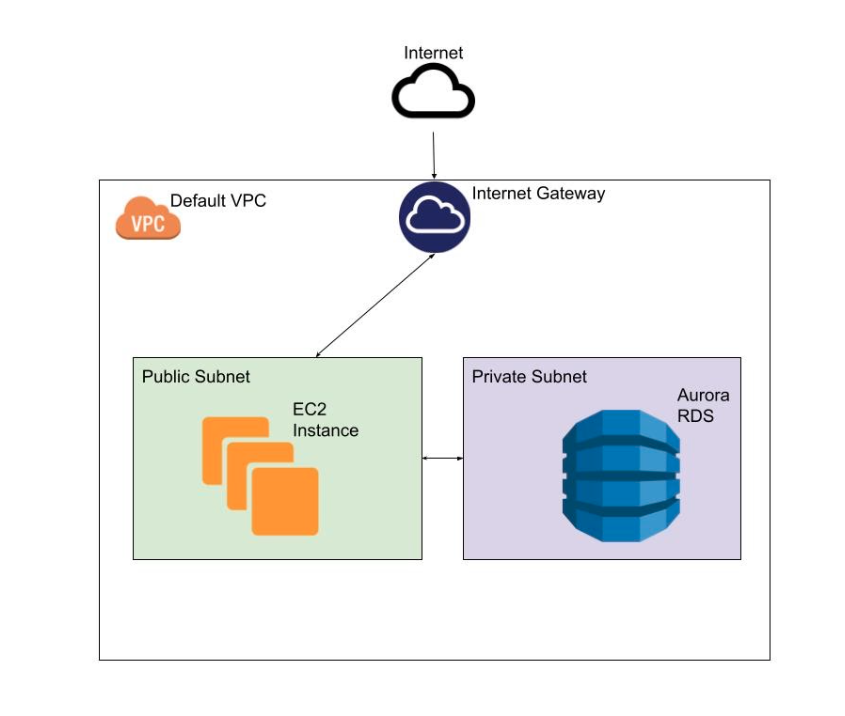
\includegraphics[width=0.9\textwidth]{architecture.png}}
\floatfoot{Note. This is the most basic and elementary recommended configuration to deploy an RDS in AWS, deploying a Database with public access to the internet is not recommended.}
\end{figure}


\subsection{Security}

AWS Defines security as their highest priority, when you sign up an account in AWS you accept that security is a shared responsibility between AWS and you. The shared responsibility model describes this as security of the cloud and security in the cloud \cite{awsSecurityModel}. Security for Amazon Aurora is managed at three levels, Authentication via AWS Identity and Access Management IAM, Network via VPC, Security Groups and the use of protocols like TLS/SSL to control the access to the database endpoints and finally authorization that can be implemented using techniques for stand-alone DB instances of MysQL or PostgreSQL such as SQL commands or database schema tables, or IAM datgabase authentication for Aurora MySQL only. 

The Internet Gateway is the one responsible for making it possible to communicate your private network with the internet, without the internet gateway you cannot connect to any of the services within your VPC from the internet,  this very important component is still part of the network, VPC. 

Exposing a Database directly to the internet is a serious security flaw, the recommended way to expose your database is limiting the database endpoint access to consumers inside your VPC, we are going to create an EC2 instance with public access to the internet so we can ssh to the instance and then send SQL commands to the database endpoint that is in the private network, EC2 instances are virtual machines running within the AWS account.
Finally, we are going to deploy the RDS database, which behind the scenes will create EC2 instances and SSD storage disks grouped in different availability zones to provide data replication and HA. 


\subsection{Deploying the Database in AWS}

Deploying all these resources manually can be tricky, and you might want to destroy the environment without the need to pick manually resources that you created before to avoid undesired charges, for these reasons we are going to use Terraform, which is an Infrastructure as Code tool that allows us to build, change e delete the components we define in our infrastructure as stated by Armon Dadgar, co-founder and CTO at HashiCorp in his Introduction to Terraform post.  

Let's get started by creating our terraform main.tf file in your project folder, I’ve created a new one called DataMiningTU60 in my home directory, feel free to clone the repository to follow along, in the main file we will be setting the region as default tags for our project. 

\begin{lstlisting}[caption=Terraform main file]
terraform {
 required_providers {
   aws = {
     source  = "hashicorp/aws"
     version = "~> 3.27"
   }
 }
 required_version = ">= 0.14.9"
}
provider "aws" {
 profile = "default"
 region  = "eu-west-1"
 default_tags {
   tags = {
     Project     = "DataMiningTU60"
   }
 }
}

\end{lstlisting}


Now let's initialize the Terraform local environment by running \textbf{\emph{\$terraform init}} command within the directory of our project.
\begin{lstlisting}[caption=Initializing Terraform local environment]
$ terraform init
Initializing the backend...  
\end{lstlisting}

\subsection{Grabbing the database infrastructure details}

It’s time to create our first Aurora DB database,  we are going to define a resource called aws\_db\_instance and name it "default" before we apply the terraform file to create the database in the cloud, we need to grab the default security group ID in the AWS Management Console VPC \ref{fig:DefaultVPC}:

\begin{figure}[hbt!]
\centering
\caption{\label{fig:DefaultVPC} Taking the Default VPC ID.}
\fbox{\includegraphics[width=0.9\textwidth]{ManagementConsole.png}}
\end{figure}

Select Security Group, and then copy the security group ID, it will be provided as input during the terraform apply execution:

\begin{figure}[hbt!]
\centering
\caption{\label{fig:SecurityGroup} Security Groups.}
\fbox{\includegraphics[width=0.9\textwidth]{SecurityGroups.png}}
\end{figure}

We will also need to create a key pair in oder to be able to connect to our bastion host, this mechanism allow us to create a pair of public and private keys with security credentials that are used to prove our identity when connecting to EC2 instances, after creating the key pair with the default parameters, save the *.pem file and modify it'’ permission with the command \textbf{\emph{\$chmod 400 your\_key\_file.pem}}

\begin{figure}[hbt!]
\centering
\caption{\label{fig:KeyPairs} Key pairs.}
\fbox{\includegraphics[width=0.9\textwidth]{KeyPairs.png}}
\end{figure}
\clearpage
Now it's time define the database resource in our \textbf{\emph{main.tf}}file:

\begin{lstlisting}[caption=Terraform main file]
variable "db_user_name" {}
variable "db_password" {}
variable "instance_key_name" {}
resource "aws_db_instance" "default" {
 allocated_storage    = 10
 engine               = "mysql"
 engine_version       = "5.7"
 instance_class       = "db.t3.micro"
 name                 = "mydb"
 username             = var.db_user_name
 password             = var.db_password
 parameter_group_name = "default.mysql5.7"
 skip_final_snapshot  = true
}
\end{lstlisting}

To create the resources we have defined, run a \textbf{\emph{\$terraform aply}}, wait for the output to get the database endpoint that we will be using to connect to the database as below:

\begin{lstlisting}[caption=Database Endpoint output]
$database_endpoint = "terraform-xxxxxxxxxxxxxxxxxxxxxxx"
\end{lstlisting}

\subsection{Playing with the Database}

Now that we already have the database endpoint, we can start playing around with our AuroraDB MySQL, but first we need to deploy our bastion host so we can connect to our database to run our SQL commands. In our main.tf file let'’s define a new resource like below, you will be asked again for the input values.

\begin{lstlisting}[caption=Database Endpoint output]
resource "aws_instance" "bastionsql" {
 ami           = "ami-05cd35b907b4ffe77" #Can be different depending on the region
 instance_type = "t2.micro"
 associate_public_ip_address = true
 key_name = var.instance_key_name
}

\end{lstlisting}

After applying the instance we will get the public IP to where we will be able to connect using our private key as shown from the command below:

\subsection{Connecting to the Database}

\begin{lstlisting}[caption=Database Endpoint output]
$ssh -i "your_key.pem" ec2-user@publicIP
\end{lstlisting}
You may need to configure an SSH inbound rule in order to allow ssh traffic from the internet, this way we will be able to reach out to our bastion host that will be used to connect to the DB instance. 

\subsection{Common DBA tasks for MySQL DB instances}

Now that we are connected to our MySQL DB instance we will describe some common DBA tasks. It may be necessary to end user sessions or queries on DB instances by using the rds\_kill and rds\_kill\_query commands: 

\begin{lstlisting}[caption=Ending user sessions or queries on DB instances]
CALL mysql.rds_kill(thread-ID)
CALL mysql.rds_kill_query(thread-ID)
\end{lstlisting}

It's also possible to skip an error on a read replica if the error is causing the read replica to stop responding and the error doesn't affect the integrity of your data, first let's verify that the error in question can be skipped, then let's skip the error.

\begin{lstlisting}[caption=Skipping read replica error.]
SHOW REPLICA STATUS\G 
CALL mysql.rds_skip_repl_error; 
\end{lstlisting}

\subsection{Working with InnoDB tablespaces}

If you are familiarized with tablespaces in MySQL, you must already know MySQL storage engine InnoDB stores table data and indexes in a tablespace. InnoDB creates a global shared tablespace that contains a data dictionary and other relevant metadata, and it can contain table data and indexes, many DBA uses InnoDB to for tuning proposal as it can create separate tablespaces for each table and partition. These separate tablespaces are stored in files and the header of each tablespace contains a number that uniquely identifies it \cite{InnoDB2021}.

Amazon RDS provides a parameter in a MySQL parameter group called innodb\_file\_per\_table which controls whether InnoDB adds new table data and indexes to the shared tablespace  or to individual tablespaces. Amazon RDS sets the default value for innodb\_file\_per\_table parameter to 1, which allows you to drop individual InnoDB tables and reclaim storage used by those tables for the DB instance. We cab set the innodb\_file\_per\_table parameter to 0 when having a large number of tables, such as over 1000 tables when using standard or general purpose SSD storage or over 10,000 tables when using Provisioned IOPS storage. When set to 0, individual tablespaces are not created and this can improve the time it takes for database crash recovery. \cite{InnoDB2021}

We can migrate multiple tablespaces to the shared tablespace by moving an InnoDB table's metadata from its own tablespace to the shared tablespace, this will rebuild the table metadata according to the innodb\_file\_per\_table parameter setting:

\begin{lstlisting}[caption=Skipping read replica error.]
ALTER TABLE table_name ENGINE = InnoDB, ALGORITHM=COPY; 
SELECT CONCAT('ALTER TABLE `', 
REPLACE(LEFT(NAME , INSTR((NAME), '/') - 1), '`', '``'), '`.`', 
REPLACE(SUBSTR(NAME FROM INSTR(NAME, '/') + 1), '`', '``'), '` ENGINE=InnoDB, ALGORITHM=COPY;') AS Query 
FROM INFORMATION_SCHEMA.INNODB_SYS_TABLES 
WHERE SPACE <> 0 AND LEFT(NAME, INSTR((NAME), '/') - 1) NOT IN ('mysql','');
\end{lstlisting}

\subsection{Creating a read replica in a different AWS Region}
As part of the InnoDB exercise, we are going to create a MySQL read replica \ref{fig:readreplica} in a different AWS Region from the source DB instance, this will improve our disaster recovery capabilities, scale read operations into an AWS Region closer to our users, and make it easier to migrate from a data center in one AWS Region to a data center in another AWS Region.

\begin{figure}[hbt!]
\centering
\caption{\label{fig:readreplica} Read Replicas cross-region.}
\fbox{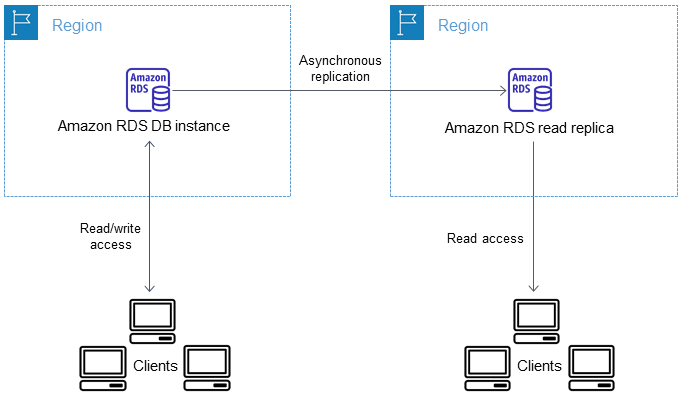
\includegraphics[width=0.9\textwidth]{read-replica-cross-region.png}}
\floatfoot{Note: \cite{readreplicaDB2021}}.
\end{figure}

To create a read replica across AWS Regions with the console:

Sign in to the AWS Management Console and open the Amazon RDS console at https://console.aws.amazon.com/rds/.

\begin{enumerate}
    \item In the navigation pane, choose Databases, MySQL DB instance that we want to use as the source for a read replica.
    \item In Actions, choose Create read replica.
    \item For DB instance identifier, enter a name for the read replica.
    \item Choose the Destination Region and the instance specifications you want to use. (The same was created before).
    \item Choose Create read replica.
\end{enumerate}

After the read replica is created, let's issue the following SQL statement for all tables that we want migrated on the replica:

\begin{lstlisting}[caption=Migrating tables on the replica.]
ALTER TABLE name ENGINE = InnoDB
\end{lstlisting}

When the ALTER TABLE statement have completed on the read replica,  the read replica will then be connected to the source DB instance and that the two instances will be in sync.

\subsection{Terminating your environment after the lab}
After performing all the tests and playing around with AuroraDB in AWS, it's time to terminate the environment so we avoid undesired charges from the cloud provider, since we have used terraform to create all the resources, we will be using the \textbf{\emph{terraform destroy}} to terminate the resources we have created as part of this demonstration. 

\begin{lstlisting}[caption=Database Endpoint output]
$terraform destroy
\end{lstlisting}

Terraform only manages the resources created and defined in our \textbf{\emph{main.tf}}file, as we have created a read replica manually, it's a good practice to confirm all the resources were terminated properly. At the end of the day the Red Replica is a resource liked with the Database we have created, and as there is a dependence relationship between these two resources, it must be terminated as part of the DB Instance termination as well, however you don't want to keep resources running in your account after completing this demonstration for any reason. 
\clearpage

To confirm whether you have any active resources, do the following. 

\begin{enumerate}
    \item Open the Billing and Cost \href{https://console.aws.amazon.com/billing}{Management console}.
    \item Choose Bills in the navigation pane.
    \item You can see the charges incurred by different services in the Bill details by service section.
    \item You can see the charges incurred in different AWS Regions in the Bill details by account section.
    \item For each service, identify the Regions where the services have incurred charges.
\end{enumerate}

To terminate the identified active resources under different services, you need to open the console for the particular service, in our case AWS RDS, enter the service name in the search bar, after opening the service console, terminate all the active resources. Be sure to check each Region where you have allocated resources.


\clearpage

\section{Comparison with Google Cloud SQL and Azure SQL Database}

Amazon Aurora, or AWS RDS according to the new branding for the AWS relational database is considered a Platform as a service (PaaS) solution, Amazon’s biggest strength is its dominance of the public cloud market in IaaS and PaaS as we can see from the Gartner Magic Quadrant for Cloud Infrastructure and Platform Services \ref{fig:MagicQuadrant}. They have the most mature enterprise-ready services that can be consumed on demand.\cite{CloudPlatformComparision}, this supremacy is also reflected in the IaaS products vast umbrella provided by Amazon as expressed by the Google trends graphics \ref{fig:Interest}.
It's important to highlight the most of the cloud providers listed in the niche players quadrant also have Cloud Database offers, with Oracle as the most mature offer for Oracle Databases which will not be covered in this study. 
\ref{fig:Compared}.
\begin{figure}[hbt!]
\centering
\caption{\label{fig:MagicQuadrant} Magic Quadrant for Cloud Infrastructure and Platform Services.}
\fbox{\includegraphics[width=0.9\textwidth]{MagicQuadrant.png}}
\floatfoot{Note: AWS is leading the quadrant since it's very first day as Cloud Provider. \cite{CloudPlatformComparision}}
\end{figure}

\subsection{Microsoft Azure SQL Database}

Azure SQL Database is the Microsoft relational database service offered by Azure, and direct competitor of AWS Aurora. The Microsoft Azure SQL Database is based on the Microsoft SQL Server engine, compatible with almost all the mission-critical capabilities of SQL Server. This managed service is designed to deliver highly available and scalable database as a service with predictable performance in the Platform as a Service (PaaS) it's equipped with data protection, disaster recovery and high availability capabilities, just like AWS RDS \cite{mazumdar2016azure}.

\textbf{Strengths compared to AWS Aurora DB}:
\begin{itemize}
    \item The main service is based on the SQL Server engine which works with most of the SQL Server tools and APIs available.
    \item Microsoft also offers Azure Database for PostgreSQL and Azure Database for MySQL.
    \item Azure has a native auto-scaling feature that scale the workload with the help of a built-in AI.
    \item Microsoft Azure SQL Database is considerably less expensive to run in comparison to AWS RDS over a month.
    \item Their native integration with SQL Server makes Azure SQL Database the best option to run Microsoft database workloads. 
    \item It has a higher score in the DB-Engines Ranking, \#14 while Aurora is placed in \#44. \cite{dbengineers2021}
        \cite{rdsvsazure2019}
\end{itemize}

\textbf{Weaknesses compared to AWS Aurora DB}:

\begin{itemize}
    \item The  Azure SQL Database API supports only 7 languages, (.Net, C\#, Java, JavaScript (Node.js), PHP, Python, Ruby) while AWS Aurora supports 19 including all already supported in Azure. 
    \item Does not have In-memory capabilities differently from AWS Aurora. \cite{dbengineers2021}
    \item SQL Azure supports focused on a subset of the features available with SQL Server, and their offer for MySQL and PostgreSQL has limited features. Amazon RDS Aurora has a better support for MySQL and PostgreSQL features as described above. 
\end{itemize}

\subsection{Google Cloud SQL}

According to Google in their public documentation, Google Cloud SQL is a fully managed relational database service for MySQL, PostgreSQL, and SQL Server that can be used to run relational databases with their native collections, configuration flags and developer ecosystem \cite{GoogleSql}. Google also has some interesting initiatives as the Cloud Spanner that was designed to replace traditional SQL databases while also serving as an OLTP (Online Transactional Processing).

\textbf{Strengths compared to AWS Aurora DB}:
\begin{itemize}
    \item Native support for SQL Server, if you want to run SQL server in AWS you need to go for the Amazon RDS for SQL Server which is a different branch comparing with Aurora with different pricing. 
    \item Integration with Cloud Spanner which allows relational and non-relational databases coexist in the same service.
\end{itemize}

\textbf{Weaknesses compared to AWS Aurora DB}:

\begin{itemize}
    \item It has a lower score in the DB-Engines Ranking, \#77 while Aurora is placed in \#44.\cite{dbengineers2021} 
    \item it supports the same only 7 languages, (.Net, C\#, Java, JavaScript (Node.js), PHP, Python, Ruby) as Azure SQL, while AWS Aurora supports 19 including all already supported in Azure. 
    \item Does not have In-memory capabilities differently from AWS Aurora. \cite{dbengineers2021}
    \item Immediate Consistency or Eventual Consistency depending on type of query and configuration, while AWS and Azure offers immediate consistency. 
\end{itemize}

\subsection{Google Trends}

With AWS RDS and Azure SQL Database services massive adoption, \cite{GoogleTrends} only a small portion of the market is left for Google Cloud SQL as we can see from the Interest over time Graph \ref{fig:Interest},\ref{fig:Compared}.. \cite{GoogleTrends}. In this session we will be comparing the three cloud databases data when it comes to trend data on the Internet. 

Google Trends data reflects searches people make on Google but also automated searches or queries that may be associated with attempts to spam our search results, the data revealed in the following graphics \ref{fig:Interest},\ref{fig:Compared}. \cite{GoogleTrends} does not represent the products adoption around the world, instead it represent the people interest based on the search people do on Google \cite{GoogleTrends}. 

\begin{figure}[hbt!]
\centering
\caption{\label{fig:Interest} Interest over time.}
\fbox{\includegraphics[width=0.9\textwidth]{InterestOverTime.png}}
\floatfoot{Note: AWS overpass Azure and Google together in the use of Relational Databases in public cloud.\cite{GoogleTrends}}
\end{figure}

When it comes to the interest breakdown per region, the massive dominance of AWS RDS is clear, with Azure leading some regions and Asia and Northen Europe, the rest of the world is still searching for ASW RDS 
\begin{figure}[hbt!]
\centering
\caption{\label{fig:Compared} Compared breakdown by region.}
\fbox{\includegraphics[width=0.9\textwidth]{ComparedByRegion.png}}
\floatfoot{Note: There are only a few regions in the world where Azure SQL Databases overpasses their competitors. \cite{GoogleTrends}}
\end{figure}

\clearpage
\section{Conclusion}

AWS RDS Aurora DB is suitable and ready to go enterprise option for those who want to migrate their on-premises relational database workload to the Cloud, with a solid security model, easy managed deployment, predictable storage, backup and recovery cloud native features, high-availability and read replicas, monitoring and more advanced options as Serverless, AWS Aurora DB is by far the most used Cloud Relational Database. 

As mentioned by professor Brendan Tierney in his Advanced Databases module for the TU60 2021/2022 course, everything in technology depends on a number of different elements, if you want to migrate a SQL Server that is currently running in Windows Server in your on-premises data center, Microsoft Azure SQL Database may be a better option, however if you are looking for a solution that allows relational and non-relational databases coexist in the same database service, Google Cloud SQL might be the best option for your case.

Most of the new features are releases first for MySQL, then to PostgreSQL, which also reflects the versions supported for each database. AWS takes more time to release new versions, when this study was been written the last General Availability version release in the community were MySQL 8.0.27 (2021-10-19, General Availability) and PostgreSQL 14.0 (2021-09-30) while AWS currently supports latest versions were MySQL 8.0.26 and PostgreSQL 13.4, which is fair considering all the concerns that an enterprise database must address in order to go live. 


\clearpage
\bibliographystyle{apacite}
\bibliography{references}
\end{document}
